\documentclass[12pt,a4paper]{report}
\usepackage[utf8]{inputenc}
\usepackage[spanish]{babel}
\usepackage[usenames, dvipsnames]{color}
\usepackage[top=0.70in, bottom=0.70in, left=0.8in,right=0.80in]{geometry}
\usepackage[pdftex]{graphicx}
\usepackage[bookmarks,  colorlinks=false]{hyperref}
\hypersetup{pdfborder = {0 0 0}}
\usepackage[final]{pdfpages}
\usepackage{float}
\usepackage{hyperref}
\usepackage[]{apacite}
\usepackage{pslatex} 
\usepackage{array}
\usepackage{setspace}
\usepackage{float}
\usepackage{enumerate}
\usepackage{longtable}
\usepackage{amssymb}
\usepackage[font=small,labelfont=bf]{caption}
\def\figurename{\textbf{Figura }}
\usepackage{listings}
\definecolor{dkgreen}{rgb}{0,0.6,0}
\definecolor{gray}{rgb}{0.5,0.5,0.5}
\definecolor{mauve}{rgb}{0.58,0,0.82}
\usepackage{fancyhdr}
\fancypagestyle{plain}{%
\fancyfoot[L]{\emph{TEC, Unidad de Ingeniería en Computación de San José}} 
\fancyfoot[R]{\thepage}
\renewcommand{\headrulewidth}{0.4pt}
\renewcommand{\footrulewidth}{0.4pt}
}
\pagestyle{fancy}

%% REEMPLAZAR POR EL NOMBRE DE SU PROYECTO %%
\rhead{\emph{Lector PDF Minimalista}}

\fancyfoot[LO,LE]{\emph{TEC, Unidad de Ingeniería en Computación de San José}}
\cfoot{}
\fancyfoot[RO, RE]{\thepage}
\renewcommand{\headrulewidth}{0.4pt}
\renewcommand{\footrulewidth}{0.4pt}
\usepackage{pgf}
\usepackage{pgfpages}


%GLOBAL SETTINGS OVER, DOCUMENT BEGINS
\begin{document}
\renewcommand\bibname{Referencias bibliográficas}
\lhead{ }

%FROM HERE YOUR PAGES START GETTING ADDED

% includes the cover page
\newpage
\begin{center}
\thispagestyle{empty}


\includegraphics[scale=1]{project/images/Firma-TEC.png}\\

\vspace{3cm}

\Large{\textbf{MANUAL TÉCNICO}}\\[0.7cm]

\LARGE{\textsc {\textbf{Lector PDF Minimalista}}}\\[0.5cm]

\vspace{1cm}
\Large{\textbf{\\ELABORADO POR}}\\[0.3cm]

\centering
\large{
Samuel Zúñiga Vega \\
Rubén Hurtado Granados \\
Andrés Alexander Feng Wu\\
Victor Gabriel Mejías Salas \\
Xotchil Daniela Rojas Fernández \\
Fabián Araya Ortega\\

}

\vspace{0.5cm}
\vspace{1cm}
\large{\textbf{SAN JOSÉ}}
\large{\textbf{\\2026}}\\
\vspace{1cm}
\newpage
\end{center}
\newpage

\begin{center}
\thispagestyle{empty}
\vspace{2cm}
\LARGE{\textbf{RESUMEN}}\\[1.0cm]
\end{center}
\thispagestyle{empty}
Este es el manual técnico para el proyecto de Lector PDF Minimalista. Su propósito es familiarizar al desarrollador con el proyecto y su diseño. Este proyecto nace de la necesidad de un lector de documentos pdf que no sea intrusivo y no sature la vista. Está necesidad fue expresada por el cliente Rodolfo Mora, él es quien recibe el producto final. Para solucionar este problema el objetivo general del proyecto es desarrollar una aplicación de escritorio para Windows que permita visualizar y modificar documentos pdf mediante una interfaz limpia, minimalista y clara.

La aplicación tiene funcionalidades de modificación de pdf (eliminar, reordenar, concatenar páginas, etc), visualización de pdf, presentación de pdf, entre otras. La implementación utiliza el framework Electron junto con bibliotecas especializadas para el manejo de pdf (PDF.js, pdf-lib). La arquitectura de la aplicación es modular, se separan las funciones en módulos independientes. El manual cuenta con instrucciones para descargar el código y desarrollar, para compilar y para desplegar en el entorno final. Al final, se comparte el aprendizaje acumulado junto con las problemáticas y limitaciones de la aplicación.\\
\textbf{Palabras clave: }Lector PDF, estilo minimalista. % adds the abstract page
\newpage

%TABLE OF CONTENTS AND LIST OF FIGURES ARE AUTOMATICALLY ADDED BY FOLLOWING COMMANDS
%ADD FIGURE OF TABLES IF YOU NEED TO, CHECK DOCUMENTATION
\pagenumbering{roman} %numbering before main content starts


%To reset the Header & Footer for TOC and LOF
\pagestyle{empty}
\addtocontents{toc}{\protect\thispagestyle{empty}}
\tableofcontents % adds Index Page

\addtocontents{lof}{\protect\thispagestyle{empty}}
\listoffigures % adds List of Figures
\cleardoublepage

%And reset back the settings we choose for Header and Footer
\pagestyle{fancy}

\newpage
\pagenumbering{arabic} %reset numbering to normal for the main content

\chapter{Introducción}

\section{Sobre este manual}

Este manual está dirigido a nuevos desarrolladores que quieren trabajar en este proyecto. Su objetivo es familiarizar a los nuevos desarrolladores con el proyecto, y brindar tanto las herramientas como la información necesaria para que puedan desarrollar sobre el proyecto de manera rápida y efectiva.

Este manual contiene el contexto del proyecto y los objetivos que quiere alcanzar (Capítulo 1), así como las funcionalidades necesarias para alcanzar dichos objetivos (Capítulo 2). También, se incluye la información sobre cómo se diseño el sistema, y cómo están implementadas las funcionalidades requeridas (Capítulo 3). Además, contiene guías para configurar el entorno de desarrollo y para desplegar el sistema (Capítulo 4). Finalmente, se incluyen reflexiones útiles sobre el proceso de desarrollo, las limitaciones del proyecto y las oportunidades de mejora que existen (Capítulo 5).

\section{Descripción y Alcance del proyecto}
\subsection{Antecedentes}

Este proyecto surge como respuesta a una necesidad directa expresada por el cliente, quien en la actualidad usa distintos lectores de PDF y manifiesta una insatisfacción con estas herramientas debido a sus interfaces sobrecargadas de utilidades, barras de herramientas y menús poco intuitivos. Además, también menciona experiencias negativas con lectores alternativos, que son más livianos, pero tienen algunos problemas de estabilidad, entre otras cosas.

Como referencia de estilo visual el cliente resaltó la interfaz que utiliza un lector desarrollado por Augmented Text Company (\url{https://www.augmentedtext.info/reader}), que corresponde a un visor sin barra de título, sin bordes intrusivos y con un estilo minimalista blanco sobre blanco agradable a la vista.

\subsubsection{Beneficiario}
El beneficiario directo del proyecto es el cliente Rodolfo Mora, quien en su labor académica maneja de forma constante documentos en formato PDF (lecturas, presentaciones exportadas y documentos legales que requieren firma), y que actualmente no cuenta con una herramienta
que combine una interfaz minimalista con las funcionalidades específicas que necesita.

\subsubsection{Importancia}
La importancia del proyecto radica en ofrecer una alternativa amigable a las aplicaciones de lectura y edición de PDF existentes en el mercado que, según lo expresado por el cliente, priorizan la cantidad de funcionalidades visibles por encima de la experiencia de lectura sobrecargando la interfaz y dificultando la concentración en el contenido. 

\subsubsection{Grupos o comunidades beneficiadas}

El principal beneficiado es el cliente. Sin embargo, dado que se contempla como un proyecto de software libre, cualquier usuario de Windows (y eventualmente Linux) que busque un lector y editor de PDF minimalista podrá beneficiarse de la herramienta desarrollada.

\subsubsection{Necesidades solventadas}

Interfaces sobrecargadas y poco intuitivas de los lectores de PDF actualmente disponibles (Adobe Acrobat, Foxit, entre otros), que dificultan una experiencia de lectura centrada en el contenido.
	

\subsection{Objetivos}

%
% Los objetivos del proyecto deben englobar el alcance total. Todo objetivo debe estar redactado respetando la siguiente estructura:

% Verbo infinitivo: Representa una acción que el equipo de desarrollo ejecutará durante el proyecto. Debe ser una acción concreta y relevante para completar el proyecto

% Objeto: Indica el objeto sobre el cual se aplicará la acción. Típicamente representa el producto esperado de la acción

% Modo: Indica parámetros por los cuales se medirá la calidad y completitud del resultado. 

% Ejemplo: Desarrollar un sistema de facturación electrónica que provea una interfaz amigable para el usuario y cumpla con los estándares impuestos por el Ministerio de Hacienda de Costa Rica. 

% Sólo puede existir un verbo infinitivo en el objetivo
% Debe ser posible medir el nivel de cumplimiento del objetivo, es decir, debe ser posible decir en cualquier momento del proyecto, cual porcentaje del objetivo se ha cumplido.

\begin{itemize}
    \item \textbf{Objetivo General}
    \begin{itemize}
        \item Desarrollar una aplicación de escritorio para Windows que
        permita visualizar y modificar documentos PDF mediante una interfaz minimalista, limpia y clara.
    \end{itemize}
    \item \textbf{Objetivos Específicos}
    \begin{itemize}
        \item Construir un visualizador de documentos pdf que muestre las páginas del documento al usuario.
        \item Desarrollar funcionalidades para hacer modificaciones simples al pdf, como eliminar, compaginar y mezclar páginas, y que se guarden en el mismo archivo o uno nuevo.
        \item Implementar la búsqueda, selección y copiado de texto en un pdf que se está visualizando.
        \item Desarrollar un modo presentación para el pdf que se está visualizando.
        \item Diseñar una interfaz minimalista con color blanco que muestre las funcionalidades de la aplicación solo cuando sea necesario, intentando mantener poca información en la pantalla para no saturar al usuario.
    \end{itemize}
\end{itemize}

\subsection{Contacto}
Para consultas y soporte, contacte a: samuelzv18@gmail.com

 % adds the introduction page
\chapter{Especificación de funcionalidad}
\section{Descripción del producto}

El producto es una aplicación de escritorio para el sistema operativo Windows. La aplicación funciona como un lector de documentos PDF, que también cuenta con funciones para hacer modificaciones. Sigue una filosofía minimalista que se refleja en la UX/UI del programa.

El lector tiene funcionalidades básicas como zoom, scroll, búsqueda de texto, salto a una página específica y selección de texto con posibilidad de copiar. Además, renderiza las páginas aplicando Lazy Loading para mejorar el rendimiento. También, tiene una sección para mostrar el outline del documento y otra para mostrar la lista de paginas del documento. Por último, el lector tiene modo de presentación en pantalla completa.

La aplicación también tiene un módulo de herramientas que modifican y editan el archivo pdf. Es posible eliminar páginas y concatenar páginas de otro archivo pdf. También se incluyen las funciones de guardar y guardar como, para conservar las modificaciones en los documentos.

La codificación para las historias de usuario es US-XXX, donde X representa el número consecutivo de historias de usuario. 

Durante el desarrollo se realizan más tareas que utilizan otro tipo de codificación. Estas tareas no se incluyen en este documento porque son de tipo  administrativo o de mantenimiento y no son relevantes para entender el producto final (así que tampoco son relevantes entre sprints).

Para las tareas sobre documentación del código se usa la codificación: DC-XXX. Para las tareas de refactorización del código se usa la codificación: FX-XXX. 

\subsection{Historias de usuario}

% La pila del producto debe actualizarla cada iteración del proyecto. Divida las historias en épicas o MVPs, de forma que sea más fácil identificar cuáles historias corresponden a cada fase.
% Añada a cada historia criterios de calidad, para esto pregúntese ¿cómo verifica el usuario que la funcionalidad está completa? ¿qué espera el usuario de 

%% PILA DE PRODUCTO %%
\begin{longtable}{|l||p{7cm}|p{4.5cm}|}

\multicolumn{3}{c}{Lector PDF minimalista}\\
\hline
\textbf{Código} & \textbf{Descripción} & \textbf{Criterios de Calidad}\\
\hline\hline
\endfirsthead
\hline
\textbf{Código} & \textbf{Descripción} & \textbf{Criterios de Calidad}\\
\hline\hline
\endhead

% Omita las historias eliminadas
% En esta tabla no coloree las historias, mantenga la última versión de la pila general del producto
\textbf{US-001} & \textbf{App minimalista}: Ocultar la información en la interfaz de usuario para dar un estilo minimalista a la aplicación. Esto se hace mediante la implementación de estilos de css que modifican la interfaz del renderer y configuraciones de la ventana de electron en el proceso principal..& Como usuario, quiero una interfaz limpia y minimalista para la aplicación, de modo que pueda enfocarme en la lectura del contenido sin distracciones visuales..\\
\hline
\textbf{US-002} & \textbf{Compaginar archivos pdf}: Compaginar 2 archivos pdf abiertos para obtener un archivo pdf resultante que es la unión del final del primer pdf con el inicio del segundo pdf. Esto se hace utilizando la biblioteca pdf-lib (en el proceso principal).  & Como usuario, quiero poder compaginar múltiples documentos o páginas, para organizar la estructura del documento final de manera lógica antes de exportarlo.\\
\hline
%\textbf{US-003} & \textbf{Mezclar archivos pdf}: Mezclar las páginas de 2 archivos pdf abiertos. Las páginas se pueden reordenan de cualquier manera. El resultado se muestra en el visualizador. Internamente se utiliza pdf-lib para manejar los archivos (en el proceso principal). & Como usuario, quiero poder intercalar o mezclar páginas de dos o más PDFs distintos, para consolidar información de múltiples fuentes en un solo archivo.\\
%\hline
%\textbf{US-004} & \textbf{Abrir varios archivos pdf}: Se puede abrir un segundo archivo pdf siempre y cuando ya exista uno cargado en memoria. El segundo pdf también se carga en memoria. Esto se hace usando la biblioteca estándar de nodejs para leer archivos junto con las funciones para mostrar dialogs de electron.  & Como usuario, quiero tener la capacidad de abrir dos archivos PDF simultáneamente (en pantalla dividida o pestañas), para comparar su contenido o trabajar con ambos de forma paralela.\\
%\hline
\textbf{US-005} & \textbf{Visualización ajustada al PDF}: Las dimensiones de la ventana se ajustan al visualizador del documento pdf. Esto se logra usando funciones de electron para modificar la ventana, y scripts en el renderer que comunican el tamaño del visualizador. & Como usuario, quiero que la aplicación renderice y adapte correctamente la visualización del documento al tamaño de mi ventana, para una experiencia ergonómica.\\
\hline
\textbf{US-006} & \textbf{Presentar PDF}:  Un pdf abierto puede mostrarse en modo presentación. Para esto se abre una nueva ventana de electron en modo pantalla completa. Esta ventana carga un visualizador diferente en el renderer que implementa las funcionalidades del modo presentación. El visualizador está implementado como una clase de javascript que internamente utiliza la biblioteca PDF.js & Como usuario, quiero activar un modo de presentación a pantalla completa, para poder exponer el contenido del documento a una audiencia ocultando los menús y herramientas.\\
\hline
\textbf{US-007} & \textbf{Eliminar páginas de un PDF}:  Eliminar páginas de un documento pdf cargado en memoria. Se elige una lista con cualquiera de las páginas del documento para ser eliminadas. Internamente se utiliza la biblioteca pdf-lib para modificar el archivo (en el proceso principal). & Como usuario, quiero poder seleccionar y eliminar páginas específicas de un PDF, para remover información irrelevante o incorrecta del documento original.\\
\hline
\hline
\textbf{US-008} & \textbf{Guardar un PDF}:  Un pdf abierto, cargado en memoria, y modificado se puede guardar en el disco en la misma ruta que estaba el archivo original (sobrescribiendo el archivo). Esto se hace usando las funciones de la biblioteca estándar de nodejs para escribir archivos .& Como usuario, quiero poder guardar los cambios realizados sobre el archivo PDF actual, para asegurar y no perder el progreso de mi edición.\\
\hline
\hline
\textbf{US-009} & \textbf{US-009: Reordenar páginas de un PDF}: La lista de páginas contiene un botón que permite reordenar las páginas arrastrándolas en la interfaz. Luego la información de la lista de páginas se transfiere al servicio de reordenamiento que utiliza pdf-lib internamente.  & Como usuario, quiero poder reordenar las páginas del documento (por ejemplo, arrastrándolas), para ajustar el flujo de lectura y la organización según mis necesidades.\\
\hline
\hline
\textbf{US-010} & \textbf{Outline de PDF}:  Desplegar un outline que contiene la estructura del documento pdf. Este outline es jerárquico. Es posible que algunos documentos pdf no tengan outline, en ese caso no se despliega un outline. Esta funcionalidad está implementada en el renderer mediante javascript, haciendo uso de la información que está en la sección del visualizador de pdf (US-015). &  Como usuario, quiero visualizar el índice (outline) del documento en un panel lateral, para comprender rápidamente la jerarquía y estructura general del texto.\\
\hline
\hline
\textbf{US-011} & \textbf{Navegar Outline}: Los elementos de la sección del outline son clickeables, cuando el usuario presiona un título del outline el visualizador de pdfs renderiza la página que contiene ese título. Esto se hace mediante scripts de javascript en el renderer. & Como usuario, quiero poder hacer clic en cualquier sección del índice (outline) y saltar directamente a esa página, para navegar ágilmente a través de documentos muy extensos.\\
\hline
\hline
\textbf{US-012} & \textbf{Guardar Nuevo PDF}:  El documento pdf abierto y cargado en memoria se puede guardar en el disco como un nuevo documento, independiente de la fuente original. Para obtener la ruta del nuevo documento se utiliza los dialogs que provee electron, y para escribir el archivo se usan las funciones de la biblioteca fs de Node.js. & Como usuario, quiero tener la opción de "Guardar como" para generar un nuevo archivo con mis modificaciones, manteniendo el PDF original intacto como respaldo. Con el fin de recuperarlo fácilmente si necesito usarlo. \\
\hline
\hline
\textbf{US-013} & \textbf{Buscar Texto}: Una combinación de teclas invoca un campo de texto donde se puede escribir la cadena de texto que se va a buscar dentro del documento pdf. Luego de escribir el visualizador del documento resalta el texto que coincide. Además del campo de texto, hay controles para navegar ppor el visualizador para encontrar todas las coincidencias. Esto se hace mediante scripts de javascript en el renderer que usan la información desplegada en el visualizador. & Como usuario, quiero utilizar una barra de búsqueda para encontrar palabras o frases específicas dentro del documento, para localizar datos puntuales sin tener que leer todo el texto.\\
\hline
\hline
\textbf{US-014} & \textbf{Abrir un PDF}:  El usuario selecciona el documento pdf que quiere abrir. Puede ser mediante un dialog del sistema, internamente implementado con funciones de la biblioteca de electron. O, puede ser mediante el arrastre del archivo a la aplicación, internamente implementado con eventos del navegador en el renderer. Sin importar el método, al final el archivo es guardado como una variable global en el proceso principal para ser usado en cualquier parte del sistema. & Como usuario, quiero poder abrir un archivo PDF desde el explorador de archivos de mi dispositivo, para acceder a su contenido dentro de la aplicación.\\
\hline
\hline
\textbf{US-015} & \textbf{Ver páginas de un PDF}:  Un pdf abierto se renderiza en el visualizador de la aplicación. Este trabajo lo hace la clase PdfViewer en base a la información del documento que está cargada en memoria. Este trabajo se hace en el renderer. Internamente se utiliza la biblioteca PDF.js. & Como usuario, quiero poder visualizar las páginas individuales del documento, para poder consumir la información que contienen.\\
\hline
\textbf{US-016} & \textbf{Copiar texto portapapeles}: Cuando se selecciona texto del visualizador (US-019) el usuario puede copiar el texto al portapapeles del sistema con un atajo del teclado. Esta funcionalidad es parte de la clase PdfViewer y proviene de la biblioteca PDF.js (ejecutado en el renderer).& Como usuario, quiero poder copiar el texto previamente seleccionado al portapapeles del sistema, para pegarlo y reutilizarlo en otras herramientas o correos.\\
\hline
\textbf{US-017} & \textbf{Zoom de un PDF}: Mediante atajos de teclado y el scroll del mouse el usuario puede cambiar el nivel de zoom del visualizador de pdf.  Esta funcionalidad es parte de la clase PdfViewer y proviene de la biblioteca PDF.js (ejecutado en el renderer). & Como usuario, quiero poder acercar (zoom in) y alejar (zoom out) la vista de la página, para visualizar detalles pequeños o evaluar la distribución completa de la hoja.\\
\hline
\textbf{US-018} & \textbf{Scroll de un PDF}: Mediante el scroll del mouse el usuario puede navegar verticalmente por el documento renderizado por el visualizador. Esta función incluye lazy loading de las páginas visualizadas para mejorar el rendimiento del programa.  Esta funcionalidad es parte de la clase PdfViewer y proviene de la biblioteca PDF.js (ejecutado en el renderer). & Como usuario, quiero poder desplazarme verticalmente (scroll) a lo largo del documento, para mantener una experiencia de lectura continua y fluida.\\
\hline
\textbf{US-019} & \textbf{Seleccionar texto}: El visualizador de pdf incluye una capa extra sobre el pdf renderizado que le permite al usuario seleccionar texto del documento. Esta funcionalidad es parte de la clase PdfViewer y proviene de la biblioteca PDF.js (ejecutado en el renderer). & Como usuario, quiero poder seleccionar bloques de texto arrastrando el cursor, como acción indispensable antes de poder copiar(US-016) o resaltar el contenido.\\
\hline
\textbf{US-020} & \textbf{Saltar a Página}: El usuario puede ingresar un número de página en el mismo elemento que se usa para desplegar la página actual. Al hacerlo, el visualizador cambia su posición vertical para que dicha página quede centrada en la pantalla y se renderice. Esta funcionalidad es parte de la clase PdfViewer y proviene de la biblioteca PDF.js (ejecutado en el renderer). & Como usuario, quiero poder ingresar un número específico de página, para saltar a esta inmediatamente sin tener que scrollear.\\
\hline
\textbf{US-021} & \textbf{Mostrar Conteo de Páginas}: Un elemento de la interfaz muestra la página actual que está renderizada en el visualizador y la cantidad total de páginas del documento.  Esta funcionalidad es parte de la clase PdfViewer y proviene de la biblioteca PDF.js (ejecutado en el renderer). & Como usuario, quiero poder la página en la que estoy en relación a la cantidad total de páginas, para saber con certeza en que parte del documento me encuentro.\\
\hline
\textbf{US-022} & \textbf{Menú Click Derecho}: Al hacer click derecho en cualquier punto de la interfaz se abre un menú contextual que despliega botones para ejecutar las funcionalidades de la aplicación. El menú contextual es construido usando funciones de la biblioteca de electron y utiliza elementos de la interfaz del sistema. Las funciones que se activan en el menú son callbacks que se inyectan desde por medio la biblioteca IPC de electron. & Como usuario, quiero poder mostrar un menú con click derecho, para acceder a todas las funcionalidades del sistema sin que estas se entrometan en el lector.\\
\hline
\end{longtable}

 % Especificación de requerimientos
\chapter{Arquitectura del sistema}
\section{Diseño general del sistema}

La aplicación está construida sobre el framework Electron, lo que influencia en gran medida la arquitectura del sistema. Una aplicación en Electron tiene un proceso de ejecución principal que corre Node.js, este se encarga de la comunicación con el sistema operativo, la creación de ventanas, entre otras cosas; utilizando las bibliotecas que provee Electron. El proceso principal a su vez puede crear uno o más procesos renderizadores (renderer process), cada uno con una ventana asignada, estos procesos corren un navegador Chromium que se encarga de desplegar la interfaz de la aplicación (aunque también puede realizar más tareas con scripts de javascript). Esto provoca que la arquitectura este dividida en 2 partes: el proceso principal y el renderer. 

En esta aplicación el renderer es el encargado de desplegar la interfaz de usuario principal donde se  visualizan los documentos pdf y los botones, y demás elementos, usados para las otras funcionalidades del sistema. El proceso principal se encarga de la creación de ventanas del sistema (como la ventana principal, diálogos del sistema, menú contextual, etc), la comunicación con el sistema operativo, las funcionalidades que modifican los documentos y cuenta con el estado de la aplicación.

El código del proyecto tiene un diseño modular basado en los módulos de javascript. En cada módulo se encuentran funciones exportadas (públicas) y las funciones no exportadas (privadas) que solo se utilizan a lo interno del módulo. Cada módulo es responsable de una funcionalidad del sistema. Usualmente un módulo del proceso principal tiene una versión análoga en el renderer.

Para comunicar el proceso principal con el proceso renderer Electron provee la biblioteca IPC (Inter-Process Comunication). En el proyecto la biblioteca se utiliza en el módulo "ipc" que trabaja como una capa de interfaz entre los servicios que provee el proceso principal y el proceso renderer. El proceso renderer se conecta con la interfaz del módulo ipc a través de un preload script que electron carga en el renderer cuando es invocado, este archivo se encuentra en la carpeta raíz del proyecto con el nombre preload.js. 

\subsection{Diagrama de dependencias}

El diagrama de dependencias muestra las dependencias entre los módulos de la aplicación. Es una forma útil de visualizar como trabajan los módulos de la aplicación entre sí y de ver que forma se relacionan. Este diagrama es generado utilizando la herramienta madge, así que muestra el proyecto tal y como está programado. También, puede resultar útil para detectar dependencias circulares o un flujo extraño dentro del programa.

El formato del diagrama es el siguiente. Cada archivo o módulo del sistema es un rectángulo, el color representa el estado de la dependencia: azul si tiene dependencias, verde si no tiene dependencias y rojo si es parte de una dependencia circular. Las flechas indican las dependencias entre módulos.

Hay un diagrama que muestra las dependencias del proceso principal (Ver figura \ref{DiagramaDependenciaMain}) y otro que muestra el proceso renderer (Ver figura \ref{DiagramaDependenciaRenderer}).

\subsubsection{Proceso principal}

\begin{figure}[H]
	\centering
	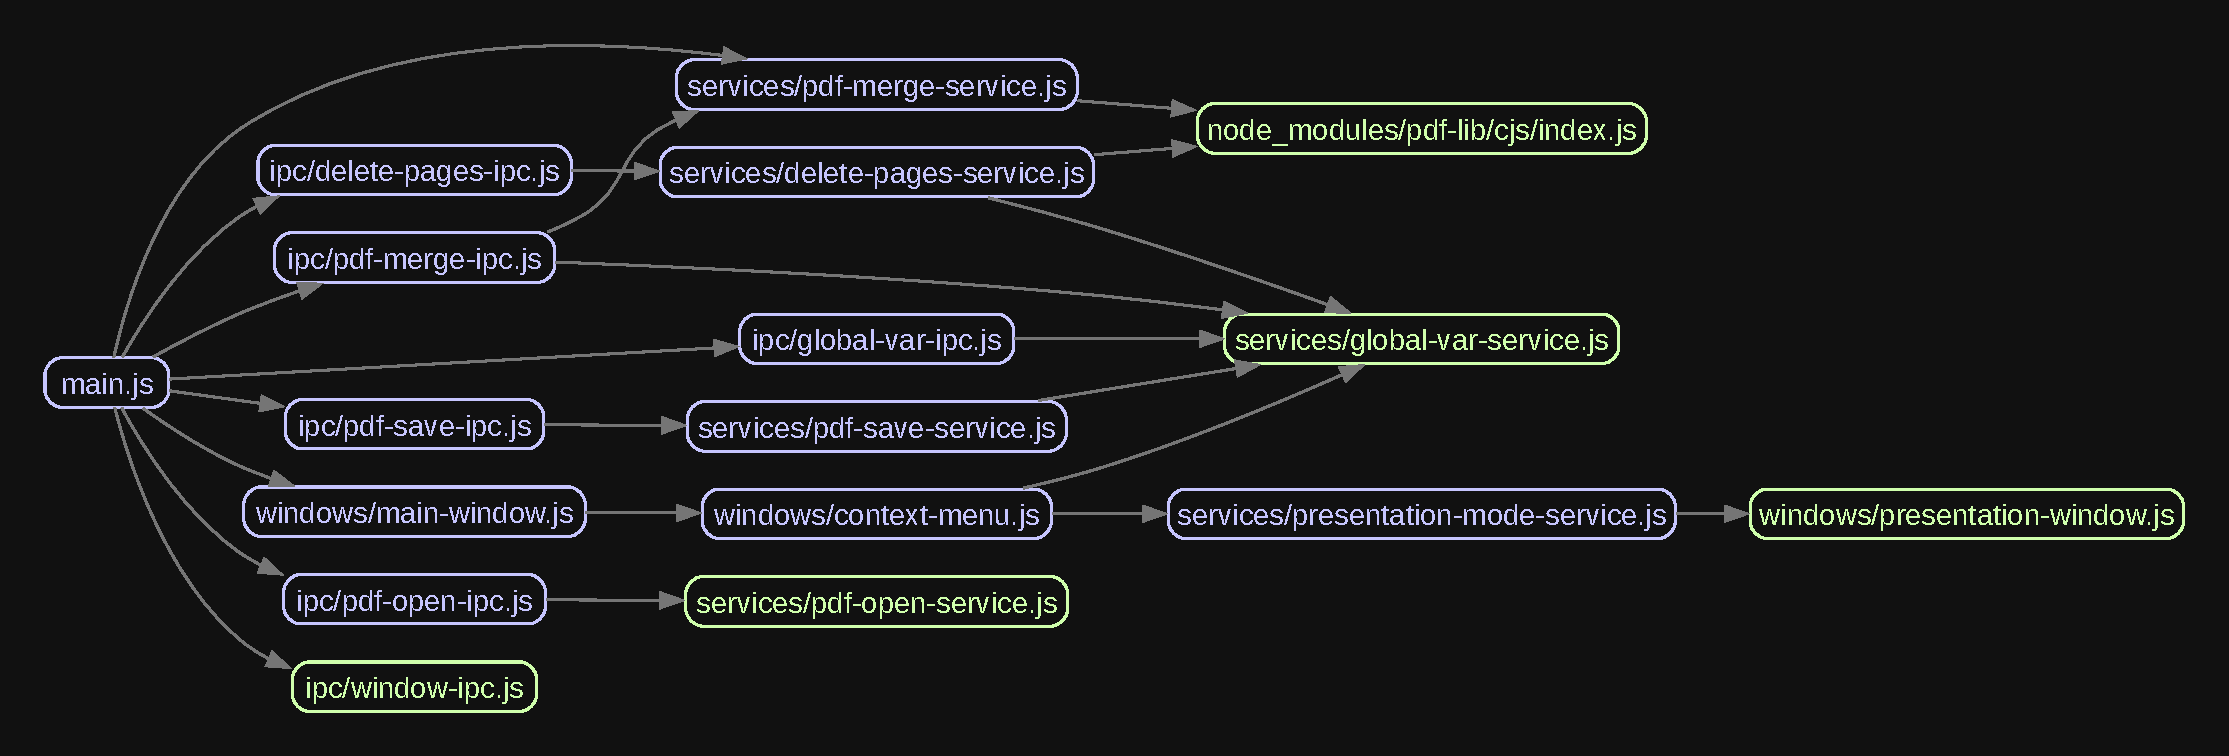
\includegraphics[width=\linewidth]{project/images/dd_main.pdf}
	\caption{\textbf{Diagrama de Dependencias: proceso principal}}
	\label{DiagramaDependenciaMain}
\end{figure}

\subsubsection{Proceso renderer}

\begin{figure}[H]
	\centering
	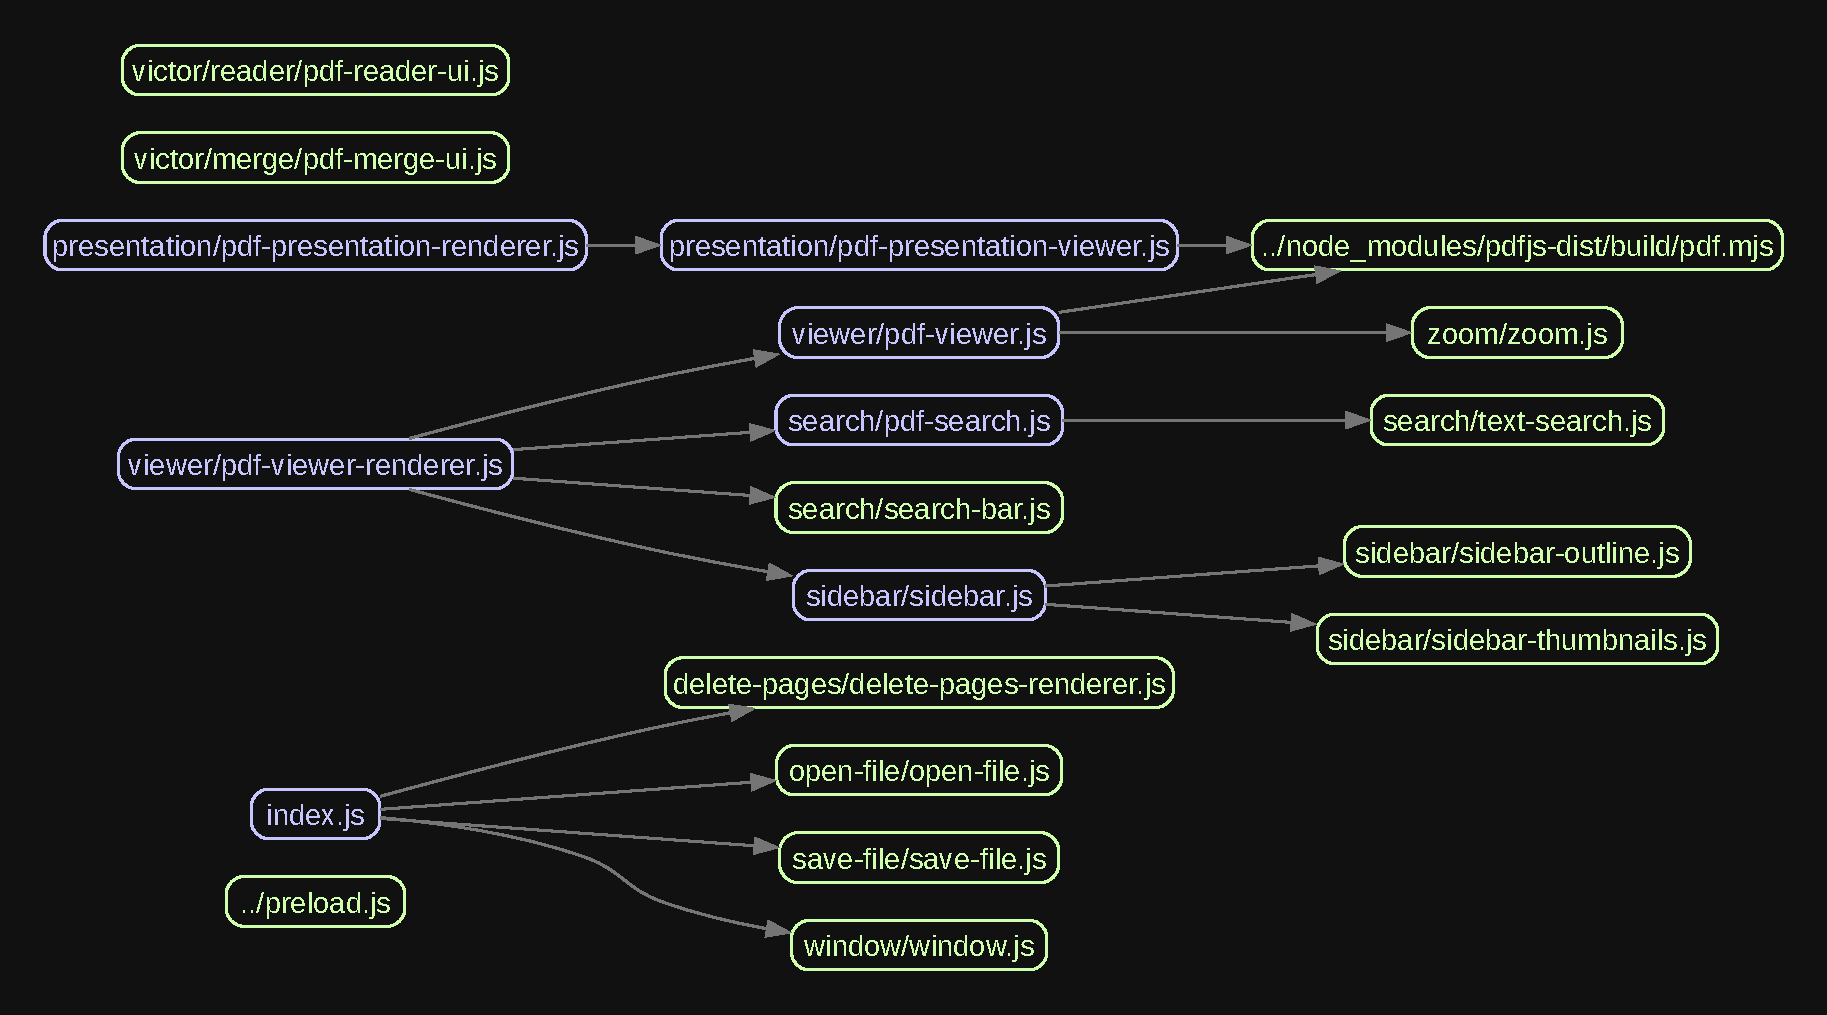
\includegraphics[width=\linewidth]{project/images/dd_renderer.pdf}
	\caption{\textbf{Diagrama de Dependencias: proceso renderer}}
	\label{DiagramaDependenciaRenderer}
\end{figure}


\subsection{Diagrama de bloques}

El diagrama de bloques muestra la organización de los módulos del proyecto y cómo se comunican entre sí de forma superficial. Este diagrama es útil para entender la estructura del proyecto ya que la jerarquía de módulos es similar a la estructura de archivos que tiene el proyecto. 

El diagrama (Ver figura \ref{DiagramaBloques}) expone 2 bloques principales: proceso principal y renderer. El bloque del proceso principal tiene el módulo "windows" que tiene ventanas del sistema, el módulo "services" que tiene módulos con funcionalidades del programa y el módulo "ipc" que expone módulos del proceso principal al proceso renderer. El bloque del proceso renderer tiene 2 módulos: index y presentation, cada corresponde a una página de la interfaz de la aplicación.

\begin{figure}[H]
	\centering
	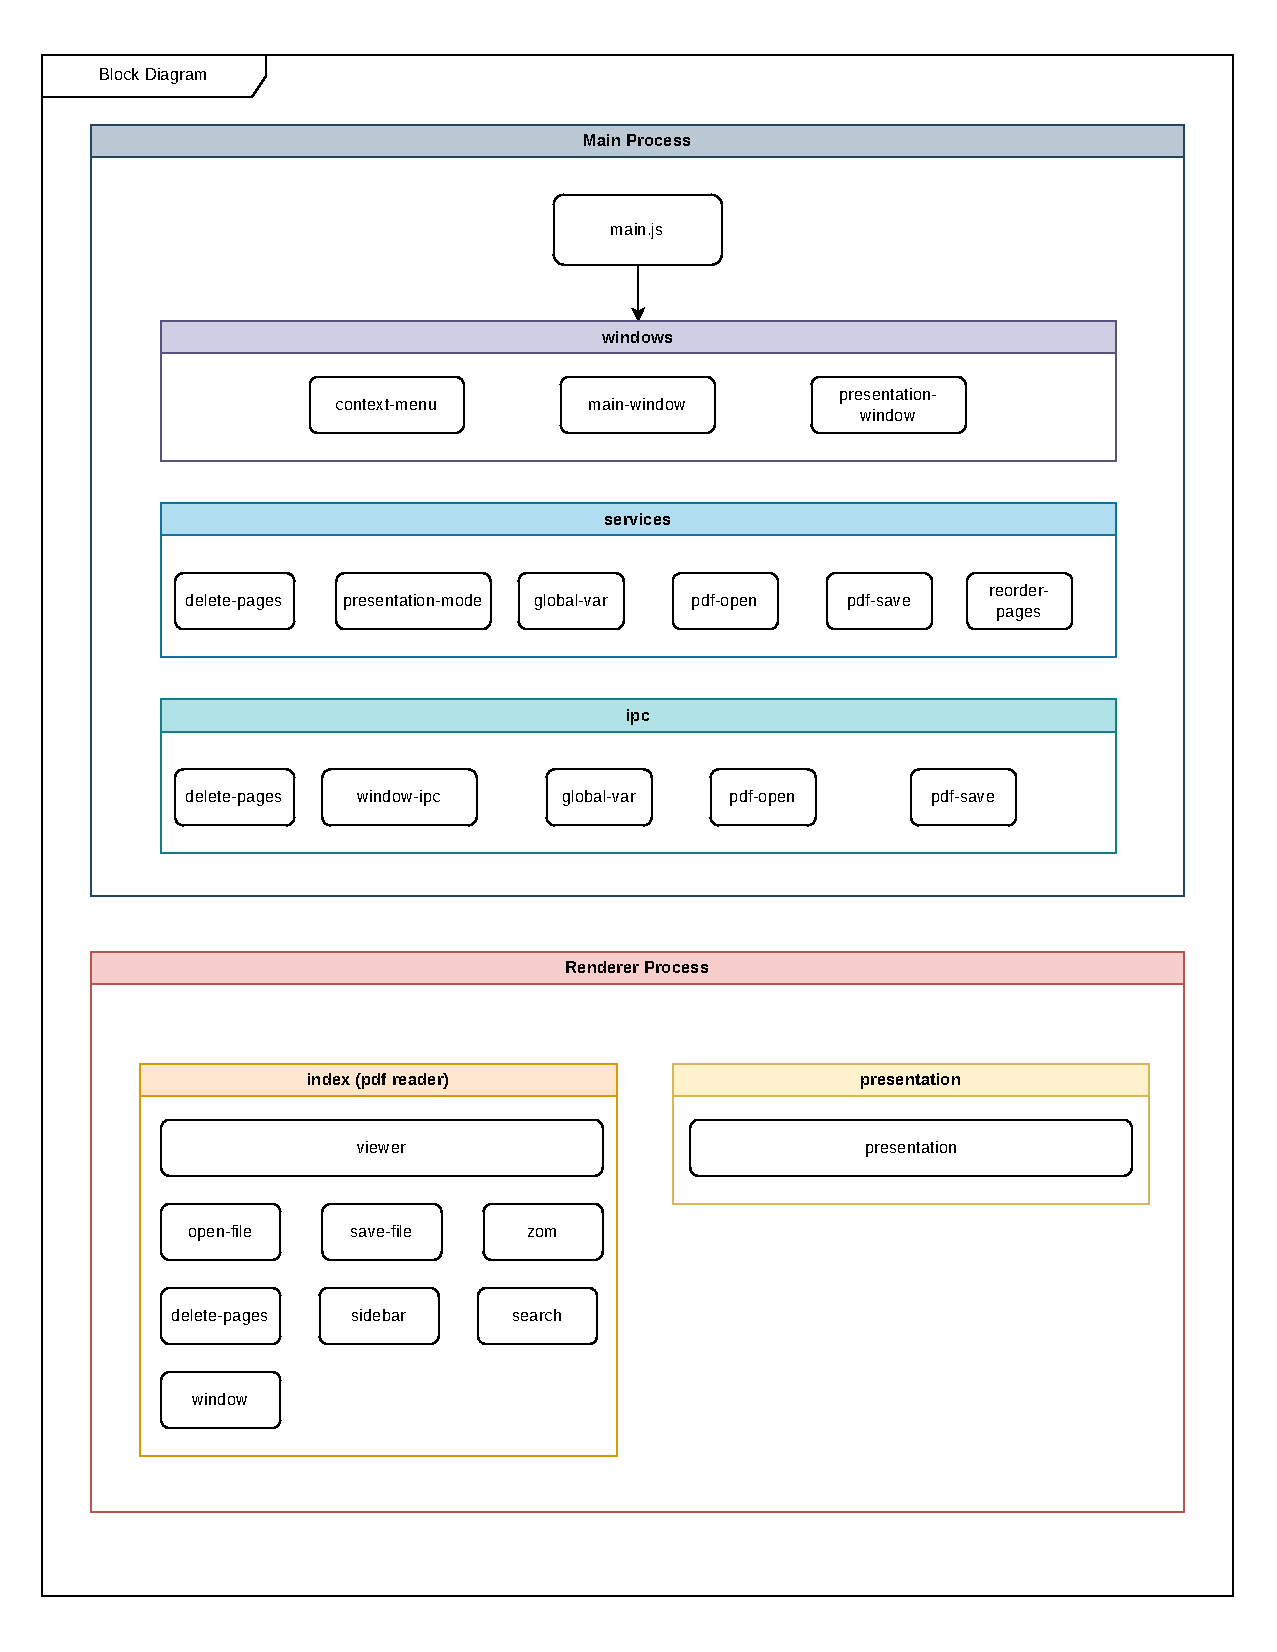
\includegraphics[width=\linewidth]{project/images/BlockDiagram.pdf}
	\caption{\textbf{Diagrama de Bloques}}
	\label{DiagramaBloques}
\end{figure}

\subsection{Diagrama de Clases}

El diagrama de clases describe las clases que existen dentro de la aplicación. El diagrama (Ver figura \ref{DiagramaClases}) muestra 2 clases. La clase PdfViewer es la encargada de mostrar el pdf dentro de la aplicación, además muestra información como número de página actual y tiene herramientas como el zoom. La clase PresentationViewer se encarga de mostrar el pdf en modo presentación.

\begin{figure}[H]
	\centering
	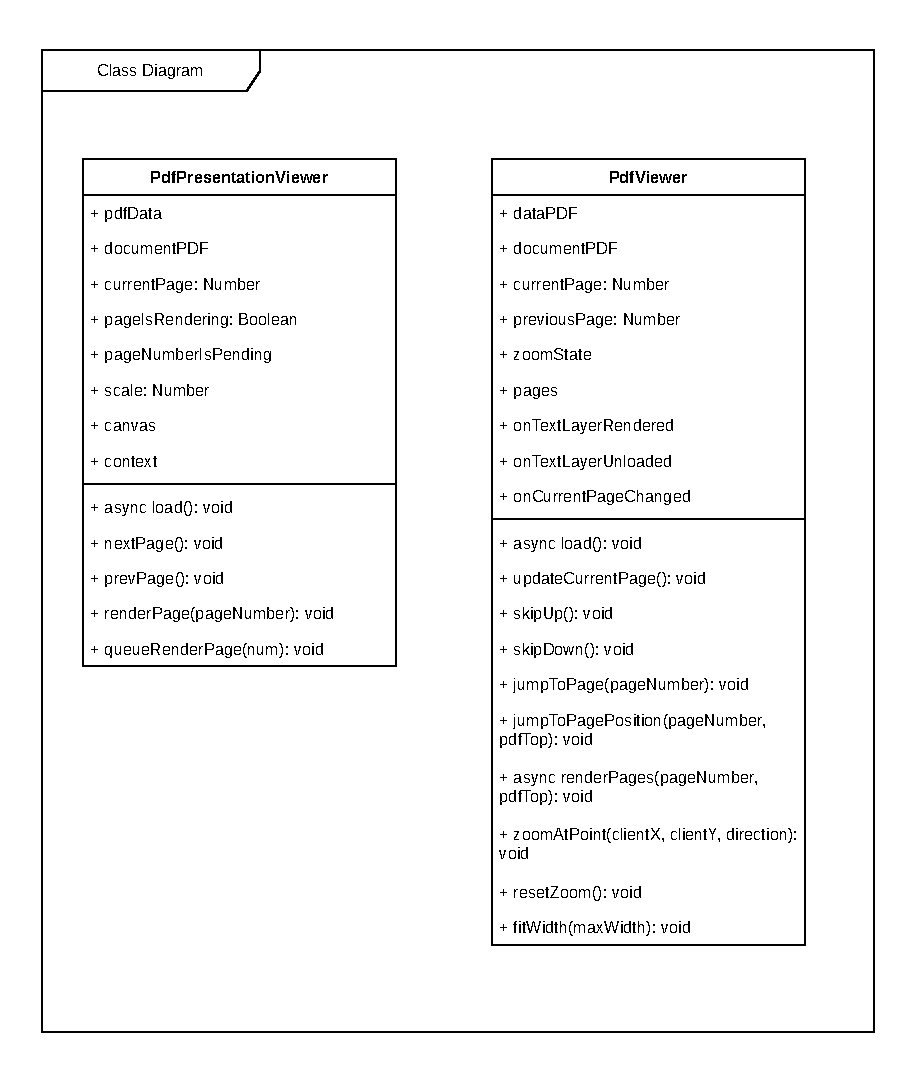
\includegraphics[width=\linewidth]{project/images/ClassDiagram.pdf}
	\caption{\textbf{Diagrama de Clases}}
	\label{DiagramaClases}
\end{figure}



 % Diseño del sistema
\chapter{Instrucciones de Instalación}

\section{Entorno de Desarrollo}

\subsection{Dependencias}
Describa el entorno de desarrollo y luego liste cada una de las dependencias en el orden en que debe instalarlas.
\begin{itemize}
    \item \textbf{Dependencia A:} Detalle las instrucciones para la primera dependencia del entorno de desarrollo
    
    \item \textbf{Dependencia B:} Detalle las instrucciones para la segunda dependencia del entorno de desarrollo
    
    %etc...
\end{itemize}

\subsection{Código fuente}
Describa los pasos necesarios para descargar y configurar el código fuente en el sistema. Incluya si lo considera necesario una descripción de archivos de configuración o scripts de preparación de base de datos.

\subsection{Despliegue en entorno de pruebas}
Describa los pasos para compilar o desplegar el sistema para probarlo en vivo en un entorno de pruebas.

\section{Entorno de Producción}

\subsection{Dependencias}
Describa las características que debe tener el entorno de producción al que se va a instalar el sistema. Considere que las dependencias del entorno de desarrollo y de producción son típicamente distintas. Por ejemplo: si está desarrollando en MEAN, en el entorno de desarrollo necesitará instalar Angular y Angular-CLI, pero en el entorno de producción no es necesario ya que debe crear un build estático de la interfaz para producción.

En el entorno de producción deberían existir menos dependencias, y puede que algunas dependencias sean distintas.
\begin{itemize}
    \item \textbf{Dependencia A:} Detalle las instrucciones para la primera dependencia del entorno de producción
    
    \item \textbf{Dependencia B:} Detalle las instrucciones para la segunda dependencia del entorno de producción
    
\end{itemize}

\subsection{Instrucciones de instalación}
Detalle qué pasos debe seguir para instalar el sistema en el entorno de producción, incluya pasos como creación de primero usuario o instalación en frío. Procure probar esta sección para garantizar que el sistema se puede instalar desde cero en un entorno de producción nuevo. % Prototipos de interfaz de usuario
%\chapter{Métodos del API}
%En esta sección detalle los métodos que tiene publicados en la sección back-end de su sistema.
%Por cada método incluya parámetros necesarios, formato de envío, y cualquier otro procedimiento necesario para comprender y utilizar correctamente su API. 
%
%Puede utilizar este como ejemplo:
%\url{https://library.vuforia.com/articles/Solution/How-To-Use-the-Vuforia-Web-Services-API.html}
%
%
 % Pruebas Capturas de pantalla
\chapter{Conclusiones y trabajo futuro}
\section{Conclusiones}

%Documente el aprendizaje acumulado durante el desarrollo del proyecto. Las conclusiones deben ser hechos concretos que puedan ser de utilidad para un lector externo que no conoce el proyecto.

El proceso renderer no cuenta con una forma de persistir datos pesados en memoria entre páginas o entre refrescos. Ya que el proceso renderer ejecuta Chromium las formas de guardar datos son el localStorage o sessionStorage, pero no son eficientes y tienen límites pequeños (<10MB). Por lo tanto, la solución a este problema es mantener la información persistente en el proceso principal y hacer que el proceso renderer la extraiga cuando lo necesita. Este método tiene la ventaja de que también permite compartir información entre varios procesos renderer (varias ventanas de la aplicación). Es importante resaltar que la comunicación entre procesos conlleva un overhead, sin embargo en este proyecto se procesan pocos datos(<1GB) y la latencia(<500ms) no es un aspecto importante.


La implementación de "lazy loading" en el visor de archivos PDFs resultó crucial. Previo a su implementación, con un archivo PDF pesado la aplicación utilizaba alrededor de 2.9GB de memoria una vez cargado el PDF completo. Tras la implementación de lazy loading el mismo archivo consumía alrededor de 700MB de memoria. El problema que surge de esto es que las páginas se deben volver a renderizar cada vez que entran en pantalla lo que puede causar que se muestren páginas en blanco hasta que carguen, aunque esto solo debería ocurrir si las páginas son muy pesadas o después de un salto con la funcionalidad de salto de página o busqueda de palabras.

A la hora de empezar un sprint es importante verificar que las historias de usuario tengan la menor dependencia entre sí. Durante el desarrollo de este proyecto, la historia de navegar el outline y la de reordenar páginas dependían completamente del sidebar, un panel lateral que contiene tanto las miniaturas de las páginas como el outline del documento. Por ende, 2 compañeros estuvieron "pegados" hasta que el desarrollador encargado del outline pudo terminar su historia de usuario. Cuando varias historias dependen de un mismo componente, conviene sacarlo a una historia aparte y hacerla de primera en el sprint.


\section{Problemáticas y limitaciones}
%Recuerde que sólo debe registrar aquellas problemáticas que el sistema TIENE, no debe mencionar problemas que aparecieron durante el desarrollo, pero que se resolvieron adecuadamente.
%Considere como problemáticas errores o comportamientos indeseables que el sistema tiene. Por ejemplo fugas de memoria, puntos en los que el sistema se cuelga, etc...
%Limitaciones por el otro lado, son cosas que el sistema NO puede hacer, ya sea por diseño o por que se quería incluir pero no fue posible. Por ejemplo la falta de multijugador por Internet es una limitación, también liste aquí las plataformas para las cuales el sistema está diseñado (sistema operativo, requerimientos mínimos, resolución recomendada, etc...).

\subsubsection{Problemáticas}

El tiempo de arranque de la aplicación es una problemática presente. Usualmente tarda más de 2 segundos en aparecer la ventana en pantalla, esto sin estar cargando ningún pdf.

La búsqueda de texto presenta errores en documentos con formato IEEE de doble columna. Al buscar un término en estos documentos, las coincidencias pueden no encontrarse o resaltarse de forma incorrecta.

\subsubsection{Limitaciones}



Los requerimientos mínimos del sistema son los siguientes:
\begin{itemize}
	\item \textbf{RAM: }200MB. Esta es la memoria para el programa base, si se carga un pdf entonces se necesita al menos una cantidad de memoria igual al tamaño del archivo.
	\item \textbf{Almacenamiento:} 250 MB. Tamaño del ejecutable de la aplicación.
	\item \textbf{Procesamiento:} Un procesador Intel i8 serie 8000 o similar. Es probable que funcione con menos procesamiento pero no ha sido probado.
	\item \textbf{Sistema operativo:} Se compilan ejecutables para los sistemas operativos Windows 11 y cualquier distribución de Linux que soporte el formato AppImage.
\end{itemize}


\section{Trabajo futuro}

Se recomienda implementar un documento de estilo global para normalizar aspectos del estilo a lo largo de la aplicación. Esto mejora la estética de la aplicación y facilita el desarrollo.

Se puede implementar una interfaz web del sistema.

Se puede implementar gestión de múltiples firmas con bloqueo de concurrencia. (Investigar acerca de Docusign).


%%%Texto explicativo, no debe aparecer en el documento final
%\section{NOTAS SOBRE LAS REFERENCIAS BIBLIOGRÁFICAS}
%En el archivo references.bib puede agregar las fuentes bibliográficas usadas en el documento en formato \emph{bibtex}.
%Puede incluir fuentes que no citó en el archivo de referencias. Aquellas que no citó automáticamente serán omitidas en la lista de referencias.
%Para citar una referencia en el texto debe usar el comando \emph{cite}. 
%
%Por ejemplo el artículo de Dean se cita usando \cite{dean2003}. 
%Note cómo los libros de Ortíz y Sánchez no salen en las referencias. 
%
%\emph{Procure eliminar esta sección de su documento}
%%%Aquí termina el texto explicativo
 % Conclusiones del informe


\bibliographystyle{apacite}
\bibliography{project/references.bib} % Referencias bibliográficas

\end{document}